\dev{Daphné Kany}{NSI Tle}

\textit{Dans cette leçon on présente le S du protocole HTTPS.}

\paragraph{Motivation : les attaques HTTP \\}
	Le protocole HTTP est en clair : les messages ne sont pas chiffrés
\begin{com}
	Lorsque Alice et Bob communiquent en utilisant le protocole HTTP, ils peuvent subir plusieurs attaques. Premièrement, leurs messages ne sont pas chiffrés. Ainsi, si Alice communique une information sensible comme un mot de passe, il peut être intercepté par un utilisateur malveillant sur le réseau. Ensuite, Alice ne vérifie jamais l'identité de Bob. Elle peut être victime d'une attaque de l'homme au milieu : Eve, un serveur malveillant, se fait passer pour Bob auprès d'Alice et pour Alice auprès de Bob.
\end{com}

	
	\paragraph{Attaque de l'espion}
	\begin{center}
		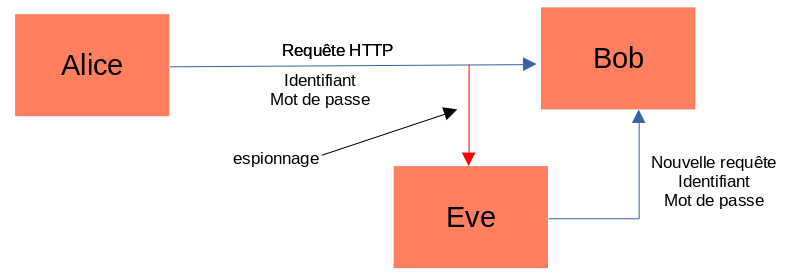
\includegraphics[scale=0.58]{Developpements/protocole https/attaque espion.png}
	\end{center}


\paragraph{}
	Comment éviter ces potentielles attaques ? 
	\begin{itemize}
		\item Communication chiffrée : Un utilisateur qui intercepte le paquet ne peut plus le lire
		\item Authentification : Alice a l'assurance qu'elle est bien en communication avec Bob.
	\end{itemize}

\paragraph{Chiffrement des données}
\begin{definition}
	Soit deux individus A et B qui communiquent un message m chiffré à l'aide d'une clef k, et déchiffrable à l'aide d'une clef k'. On dit que le chiffrement est symétrique si k = k', et asymétrique sinon
\end{definition}

\begin{example}
	Le chiffrement de César, qui consiste à décaler les lettres du message de k caractères, est un chiffrement symétrique.
\end{example}

\begin{com}
Problème : Avant d'utiliser une clef commune, A et B doivent se la communiquer. S'ils le font en clair, un espion pourra plus tard déchiffrer leurs messages. D'où l'intérêt des chiffrements asymétriques.
\end{com}

\paragraph{Chiffrement asymétrique\\}
	Le chiffrement RSA est un chiffrement asymétrique très utilisé. Les utilisateurs A et B disposent chacun d'une clef publique $K_{A}^{pub} ; K_{B}^{pub}$ et d'une clef privée  $K_{A}^{priv} ; K_{B}^{priv}$ qu'ils ne communiquent jamais. \\
	Les messages ont la particularité d'être chiffrable et déchiffrable par les deux clefs : \\
	$$dechiffre(K_{A}^{priv}, chiffre(K_{A}^{pub}, m)) = dechiffre(K_{A}^{pub}, K_{A}^{priv},m)) = m$$
	\begin{center}
		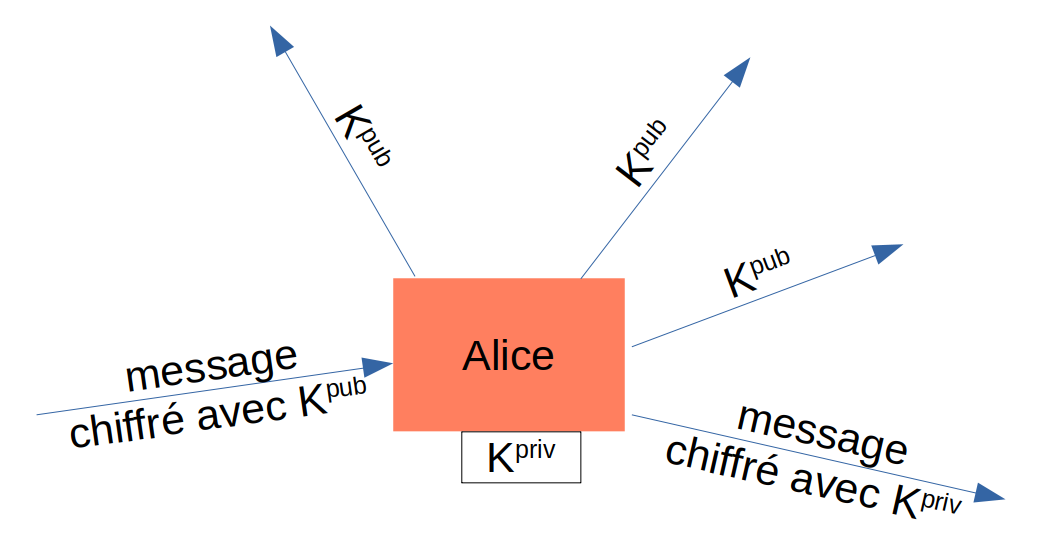
\includegraphics[scale = 0.38]{Developpements/Protocole HTTPS/cle_publique.png}
	\end{center}

Alice peut donc envoyer des messages qu'elle seule peut envoyer et elle peut recevoir des messages qu'elle seule peut décoder.

\paragraph{Idee} On peut alors utiliser cela :
\begin{center}
	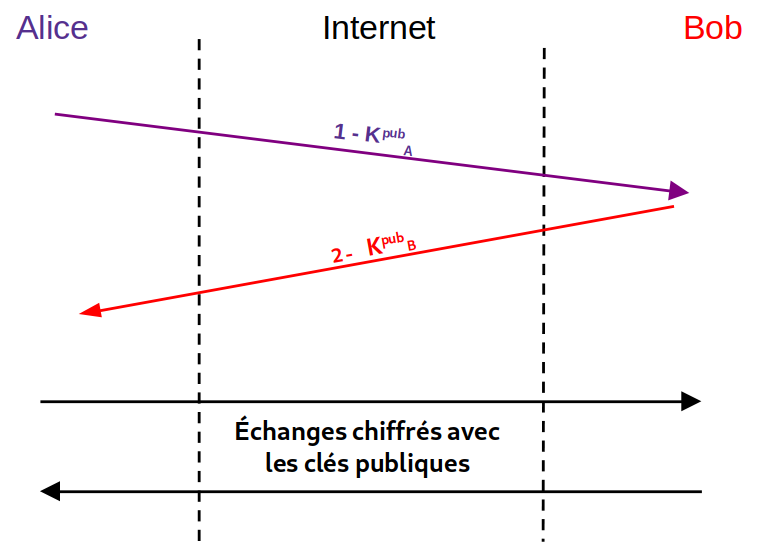
\includegraphics[scale = 0.5]{Developpements/Protocole HTTPS/protocole1.png}
\end{center}


\paragraph{Probleme} La fonction de chiffrement asymetrique est lourde à calculer. On l'utilise donc au début d'une communication, pour partager une clef symétrique qui servira au chiffrement des messages ultérieurs.

\begin{center}
	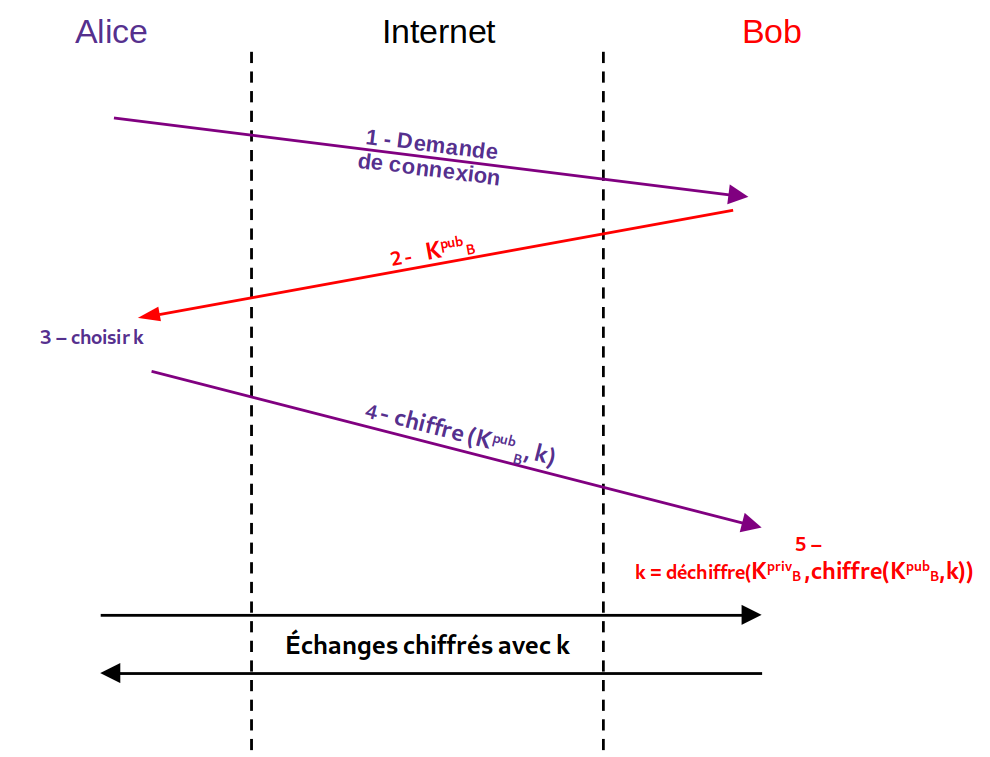
\includegraphics[scale = 0.5]{Developpements/Protocole HTTPS/protocole2.png}
\end{center}



\paragraph{Attaque de l'homme au milieu}
\begin{center}
	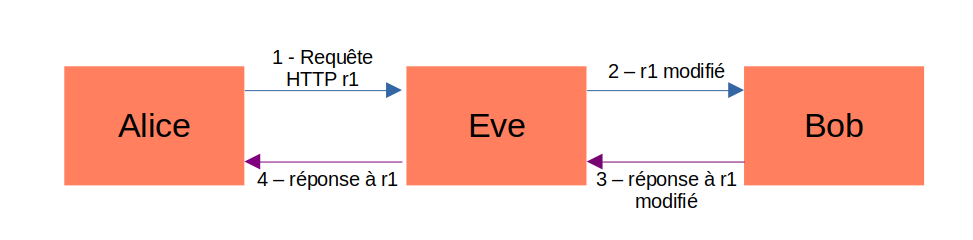
\includegraphics[scale=0.5]{Developpements/protocole https/homme_du_milieu.png}
\end{center}

\paragraph{Certificat\\}
Le protocole HTTPS repose sur l'authentification du serveur grâce à un certificat délivré par un tiers de confiance (une autorité de certification ou AC). Parmi les AC, on trouve des entreprises spécialisées, des associations à but non lucratifs et des états.  \\
Ces certificats sont créés à partir des clefs RSA des participants. 
\\
\begin{center}
	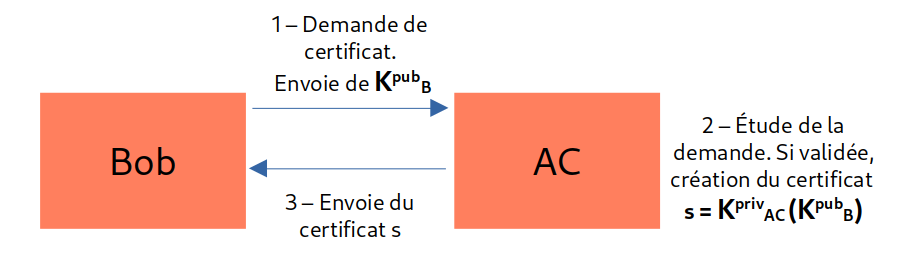
\includegraphics[scale=0.5]{Developpements/protocole https/certificat.png}
	{Obtention d'un certificat}
\end{center}

\begin{com}
	Les certificats ont des dates de péremption (validité de qq mois à qq années) et doivent donc être redemandés régulièrement. Les AC sont très surveillées et peu nombreuses : Modzilla en reconnait une centaine.
\end{com}

\begin{com}
	\textbf{Protocole HTTPS}
	\begin{itemize}
		\item Etape 1 : Alice envoie un message initial "Demande de connexion" et indique les différents algorithmes cryptographiques qu'elle supporte. 
		\item Etape 2 : Le serveur Bob lui répond en envoyant son certificat $s = K_{AC}^{priv}(K_{B}^{pub}) $et sa clef publique $ K_{B}^{pub}$.
		\item Etape 3 : Alice vérifie le certificat grâce à la clef publique de l'AC qu'elle doit posséder. 
		\\ $K_{AC}^{pub}(K_{AC}^{priv}(K_{B}^{pub})) = K_{B}^{pub}$
		\item Etape 4 : Alice utilise la clef publique de Bob pour lui communiquer de façon chiffrée une clef symétrique de chiffrement k. Elle lui envoie donc $K_{B}^{pub}(k)$
		\item Etape 5 : Bob déchiffre k grâce à sa clef privée.
	\end{itemize}
\end{com}

\begin{center}
	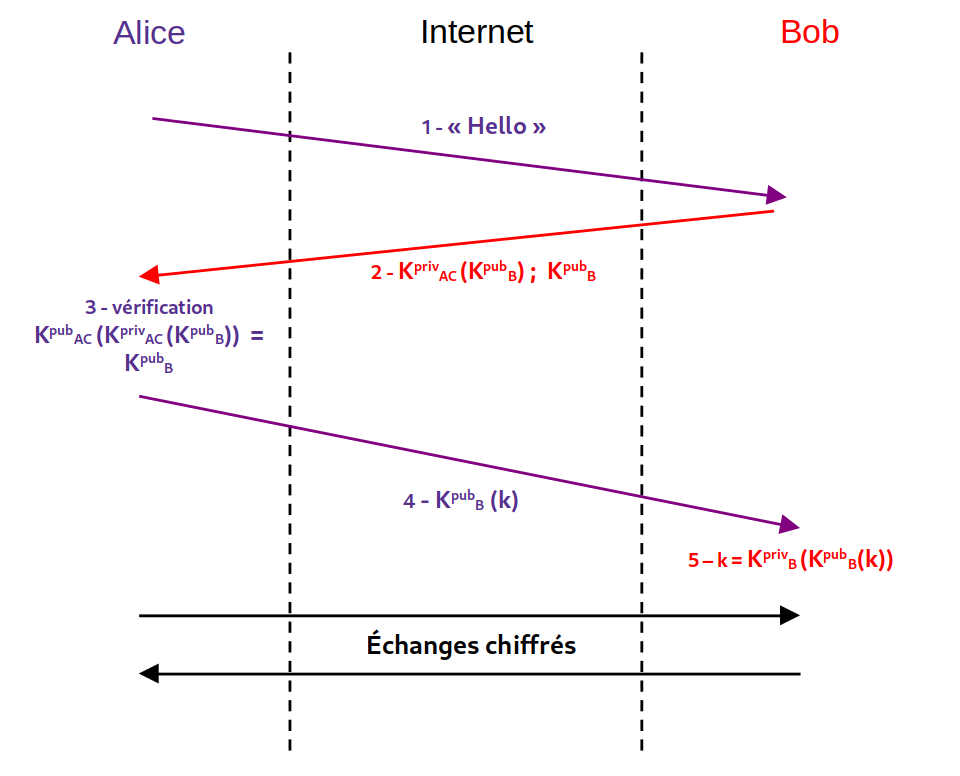
\includegraphics[scale=0.5]{Developpements/protocole https/https.png}
	{Authentification HTTPS}
\end{center}

La suite du protocole est identique à HTTP, mais tous les messages sont chiffrés avec k.

\paragraph{Robustesse aux attaques \\}
Dans le cas d'une attaque de l'homme au milieu, Eve ne connaît pas la clef privée de Bob et ne pourra donc pas récupérer la clef symétrique k envoyée par Alice. \\
Si dans le réseau un individu intercepte les messages, il ne pourra pas non plus récupérer k. Les données sont protégées. 
